\documentclass[a4paper,12pt]{exam}

\usepackage[T1]{fontenc}
\usepackage[utf8]{inputenc}
\usepackage[dutch]{babel}
\usepackage{cmbright}

\usepackage{graphicx}
\usepackage[export]{adjustbox}
\usepackage[detect-none, list-final-separator={ en }, per-mode=symbol,
            retain-explicit-plus, output-decimal-marker={,},
            exponent-product={\cdot}, range-phrase={ tot }]{siunitx}
\usepackage[font={small,sf},labelfont={bf},labelsep=endash]{caption}
\usepackage{MnSymbol}

\graphicspath{{figures/}}

\newcommand{\figref}[1]{Figuur~\ref{#1}}
\renewcommand{\eqref}[1]{Vergelijking~\ref{#1}}
\newcommand{\tabref}[1]{Tabel~\ref{#1}}

\newcommand{\rchisq}{\ensuremath{\tilde\chi^2}}

\header{\bfseries Toets data-analyse}{\bfseries NP2}{\bfseries Versie 1}
\footer{}{}{\bfseries\iflastpage{Einde $\blacksquare$}{Lees verder $\filledmedtriangleright$}}


\begin{document}
\suppressfloats[t]
\begin{questions}
  \uplevel{Anouk wil de valversnelling $g$ bepalen met de slingerproef. Zij bevestigt daartoe een massieve bol aan een dun koord en meet voor verschillende lengtes $L$ van het koord 20 slingeringen. Het resultaat van de metingen is weergegeven in \tabref{tab:metingen}. De lengtes zijn gemeten met een te verwaarlozen onzekerheid. De onzekerheid in de tijdmeting is \SI{0,2}{\second}.}

  \begin{table}
    \centering
    \caption{Gemeten slingertijd als functie van de lengte van de slinger.}
    \label{tab:metingen}
    \begin{tabular}{
        l
        l
        % *{9}{S[table-number-alignment=center,
        %        table-figures-integer=2,
        %        table-figures-decimal=1]}
        % S[table-number-alignment=center,
        %   table-figures-integer=3,
        %   table-figures-decimal=1]
        *{10}l
      }
      $L$ & [\si{\centi\meter}] & 10 & 20 & 30 & 40 & 50 & 60 & 70 & 80 & 90 & 100 \\
      $T$ & [\si{\second}] & 0,75 & 0,97 & 1,16 & 1,39 & 1,47 & 1,59 & 1,72 & 1,85 & 1,93 & 2,04 \\
    \end{tabular}
  \end{table}

  \uplevel{Anouk verwacht het volgende verband:
  \begin{equation}
    T = 2\pi\sqrt{\frac{L}{g}}.
    \label{eq:slingertijd}
  \end{equation}
  Met behulp van Origin heeft Anouk de meetgegevens uitgezet in een grafiek en gefit aan \eqref{eq:slingertijd}. Zie \figref{fig:metingen-fit}.
  }
  \begin{figure}
    \centering
    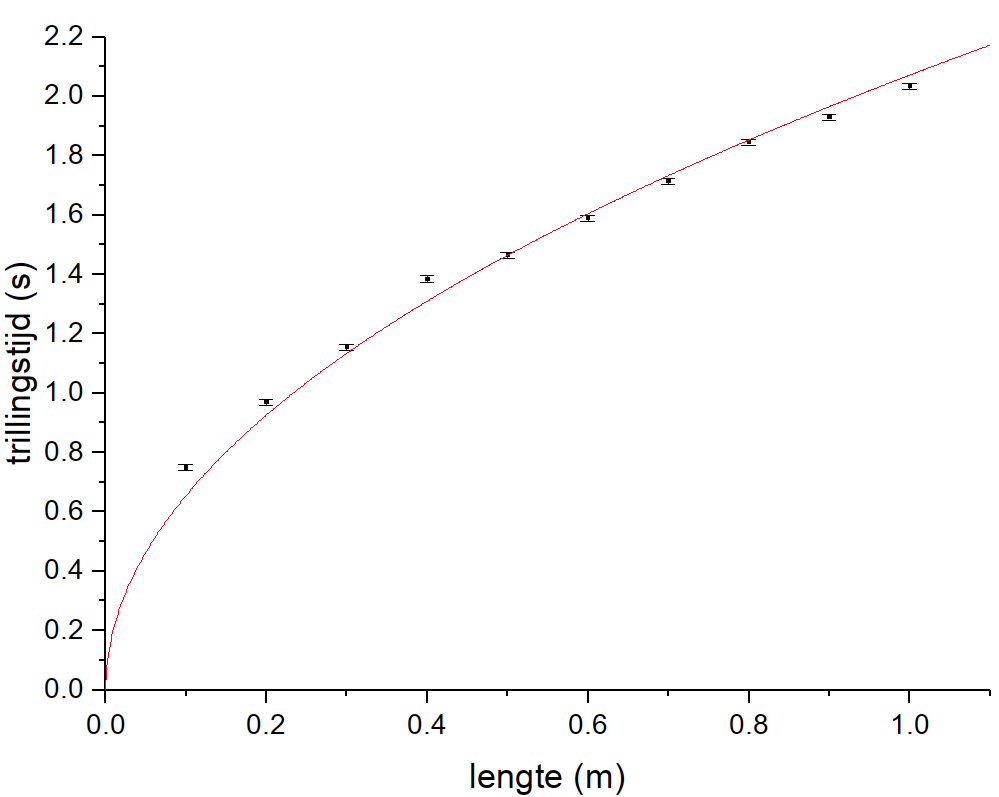
\includegraphics[width=.6\linewidth,valign=t]{fit-slingertijd}
    \hfill
    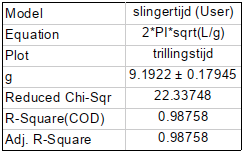
\includegraphics[width=.3\linewidth,valign=t]{fit-parameters-slingertijd}
    \caption{De trillingstijd als functie van de lengte van een slinger.}
    \label{fig:metingen-fit}
  \end{figure}
  \question Geef de gevonden waarde voor de valversnelling $g$, inclusief de onzekerheid, in de juiste notatie.
  \uplevel{Op grond van deze grafiek besluit Anouk dat haar verwachting niet klopt en dat er waarschijnlijk meer aan de hand is.}
  \question Geef daarvoor twee redenen.
  \uplevel{Anouk vermoedt dat ze de lengtes niet goed heeft opgemeten en dat er sprake kan zijn van een systematische fout. Ze besluit nu de data te fitten aan het volgende verband:
  \begin{equation}
    T = 2\pi\sqrt{\frac{L + L_0}{g}},
    \label{eq:slingertijd-offset}
  \end{equation}
  met $L_0$ de systematische fout in de lengte $L$. De resultaten staan in \figref{fig:metingen-fit-offset}.}
  \begin{figure}
    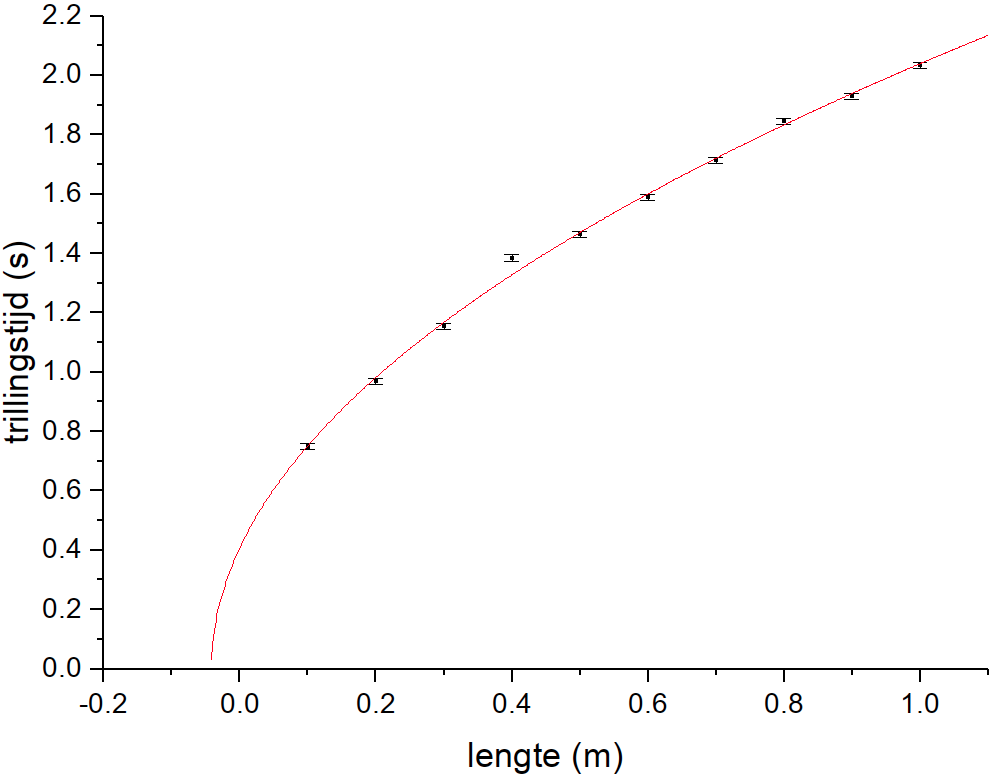
\includegraphics[width=.6\linewidth,valign=t]{fit-slingertijd-offset}
    \hfill
    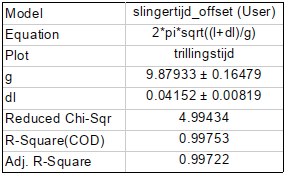
\includegraphics[width=.3\linewidth,valign=t]{fit-parameters-slingertijd-offset}
    \caption{De trillingstijd als functie van de lengte van een slinger, met systematische fout.}
    \label{fig:metingen-fit-offset}
  \end{figure}
  \uplevel{Anouk is nog steeds niet erg tevreden over de fit. De fit ziet er op zich goed uit, maar ze maakt zich zorgen over haar metingen bij een lengte van \SI{40}{\centi\meter}. Ze denkt dat ze die meting verkeerd heeft opgeschreven.}
  % \question Bereken de trillingstijd die ze theoretisch zou verwachten bij een lengte van \SI{40}{\centi\meter}. Negeer daarbij de onzekerheid.
  \question Aangenomen dat \eqref{eq:slingertijd-offset} inderdaad geldig is, bereken dan de kans op een meting bij \SI{40}{\centi\meter} die minstens zo afwijkend is als de waarde die Anouk heeft gevonden. Maak gebruik van Appendix B in Taylor.
  \uplevel{Anouk besluit het meetpunt te verwijderen, en de fit opnieuw te doen. Ze vindt nu een \rchisq-waarde van \num{0.6}.}
  \question Bereken de bijbehorende $p$-waarde en leg uit wat de betekenis is van een $p$-waarde. Maak gebruik van Appendix D in Taylor.
\end{questions}
\end{document}
